% !Mode:: "TeX:UTF-8"

\titlepage

% \begin{frame}{说在前面}
% 	\linespread{1.5}
% 	  \begin{itemize}[<+-|alert@+>]
% 	    \item 过往的作业不订正、不补齐的不予批改,打分不超过\,\ba{C}
% 	    \item 不交作业的默认记为\,\ba{D}
% 	    \item 需要换作业本的,请“移植”照片,写清楚个人信息
% 	    \item 请自行完成SPOC课程中的测试
% 	    \item 第二次单元测试即将发布,成绩记入期末总成绩
% 	  \end{itemize}
% \end{frame}

% \begin{frame}{需要注意的问题}
% 	\linespread{1.5}
% 	  \begin{itemize}%[<+-|alert@+>]
% 	    \item L'Hospital法则
% 	    \begin{itemize}
% 	      \item \it 只能应用于“$\df{\bm{0}}{\bm{0}}$”
% 	      和“$\df{\bm{\infty}}{\bm{\infty}}$”型
% 	      \item \it 及时使用无穷小代换进行简化
% 	      \item \it 不正规的符号:\b 
% 	      $\xlongequal{\footnotesize\mbox{“L”}}$、
% 	      $\xlongrightarrow{\footnotesize\mbox{“L'Hospital法则”}}$、
% 	      $\df{\bm{0}}{\bm{0}}$、$\df{\bm{\infty}}{\bm{\infty}}$
% 	    \end{itemize}
% 	    \item Taylor公式
% 	    \begin{itemize}
% 	      \item \it Taylor多项式不包含余项
% 	      \item \it 合并同次幂的系数
% 	      \item \it 尽量按照幂次由低到高排列,最后写余项
% 	    \end{itemize}
% 	  \end{itemize}
% \end{frame}

\begin{frame}{出现的问题}
	\linespread{1.5}
	  \begin{itemize}%[<+-|alert@+>]
	    \item 错误的推导
	    \begin{itemize}
	      \item \it\b $F(x)=\df{f(x)-f(a)}{x-a}=f'(\xi)\;\Rightarrow\;
	      F'(x)=f''(\xi)$
	      \item \it\b $\limx0\df{f''(x)}{|x|}=0\;\Rightarrow\; f''(0)=|x|=0$
	      \item \it\b $\limx0\df{f''(x)}{|x|}=0\;\Rightarrow\; f''(x)=|x|>0$
	      \item \it\b $\limx{a}F(x)=f'(x)$\pause
	    \end{itemize}
	    \item 自己发明的符号和说法
	    \begin{itemize}
	      \item \it\b $g''|_{x\to\frac12^+}$
	      \item \it\b $R((x-3)^n)$
	      \item \it\b $f(x)$在$x\to0^-$递减,在$x\to0^+$递增
	    \end{itemize}
	  \end{itemize}
\end{frame}

\section{3.3 Taylor公式}

\begin{frame}
	\linespread{1.5}
	\ba{4.计算如下极限:}
	\pause
	
% 	\bigskip
	
	\small 解:
	(1)$\limx{+\infty}(\sqrt[3]{x^3+3x^2}-\sqrt[4]{x^4-2x^3})$
	
	\quad$=\limx{+\infty}x\left(\sqrt[3]{1+\frac3x}
	-\sqrt[4]{1-\frac2x}\right)
	\quad =\lim\limits_{y\to0}\df{\sqrt[3]{1+3y}
	-\sqrt[4]{1-2y}}{y}$
	
	\quad$=\lim\limits_{y\to0}\df{1+\frac133y-1-\frac14(-2y)+\circ(y)}y=\df32$
	
	\pause	
	(2)$\limx0\df{\cos x-e^{-\frac{x^2}2}}{x^2[x+\ln(1-x)]}$
	
	\quad$=\limx0\df{1-\frac{x^2}2+\frac12\frac{x^4}{4!}-1+\frac{x^2}2
	-\frac{x^4}{4}+\circ(x^4)}{x^2(x+(-x)-\frac{x^2}2+\circ(x^2))}
	=\df16$
	
	\pause
	(3)
	$\limx0\df{1+\frac12x^2-\sqrt{1+x^2}}{(\cos x-e^{x^2})\sin x^2}$
	
	\quad$=\limx0\df{1+\frac12x^2-\left(1+\frac12x^2-\frac18x^4+\circ(x^4)\right)}
	{\left(1-\frac{x^2}2-1-x^2+\circ(x^2)\right)x^2}=-\df1{12}.$
\end{frame}

\begin{frame}
	\linespread{1.5}
	\ba{4.计算如下极限:}
	\pause
	
% 	\bigskip
	
	\small 解:
	(4)$\limx{+\infty}\left[\left(x^3-x^2+\df{x}2\right)e^{\frac1x}
	-\sqrt{x^6+1}\right]$
	
	\quad$=\lim\limits_{y\to0^+}\df{\left(1-y+\frac12y^2
	\right)e^y-\sqrt{1+y^6}}{y^3}$
	
	\quad$=\lim\limits_{y\to0^+}\df{\left(1-y+\frac12y^2
	\right)\left(1+y+\frac{y^2}2+\frac{y^3}6+\circ(y^3)\right)
	-\left(1+\circ(y^3)\right)}{y^3}$
	
	\quad$=\lim\limits_{y\to0^+}\df{\frac16y^3+\circ(y^3)}{y^3}=\df16.$
\end{frame}

\begin{frame}
	\linespread{1.5}
	\ba{5.应用关于$(x-1)$的$3$阶Taylor公式计算$\sqrt[3]{2}$的近似值,并估计其误差。
	}\pause
	
	\bigskip
	
	\small 解:\it 
	由Taylor公式,存在$\xi$介于$1$和$x$之间,使得
	\begin{align*}
		&\sqrt[3]x=[1+(x-1)]^{\frac13}\\
		&=1+\df13(x-1)
		+\df13\cdot\df{-2}3\cdot\df{(x-1)^2}2
		+\df13\cdot\df{-2}3\cdot\df{-5}3\cdot\df{(x-1)^3}6\\
		&\quad+\df13\cdot\df{-2}3\cdot\df{-5}3\cdot\df{-8}3
		\cdot\df{\xi^{\frac13-4}}{4!}(x-1)^4\\
		&=1+\df{x-1}3-\df{(x-1)^2}9+\df{5(x-1)^3}{81}
		-\df{10(1+\xi)^{\frac13-4}}{243}(x-1)^4,
	\end{align*}
	
	\pause
	
	带入$x=2$即得
	$\sqrt[3]2\approx\df{104}{81},$
	注意到$1\leq\xi\leq 2$,故计算误差$\left|\df{10\xi^{\frac13-4}}{243}\right|
	\leq\df{10}{243}$。
	\hfill$\Box$
\end{frame}

\begin{frame}
	\linespread{1.5}
	\ba{5.应用$3$阶Taylor公式计算$\sqrt[3]{30}$的近似值,并估计其误差。
	}\pause
	
	\bigskip
	
	\small 解:\it 
	$\sqrt[3]{30}=3\sqrt[3]{1+\frac19}$,由Taylor公式,对任意$x>0$
	存在$\xi\in(0,x)$,使得
	$$(1+x)^{\frac13}=1+\df13x-\df19x^2+\df5{81}x^3
	-\df{10(1+\xi)^{\frac13-4}}{243}x^4,$$
	
	\pause
	带入$x=\frac19$,计算可得$\sqrt[3]{30}\approx\df{61160}{19683}\approx
	3.10725$,
	注意到$0<\xi<\frac19$,故计算误差
	$$3\left|\df{10(1+\xi)^{\frac13-4}}{243}
	\df1{9^4}\right|\leq3\left|\df{10}{243}\df1{9^4}\right|=\df{10}{531441}
	\approx 1.88\times10^{-5}.$$
	\hfill$\Box$
\end{frame}

\begin{frame}
	\linespread{1.5}
	\ba{6.已知$f(x)$在$x=0$附近二阶可导,且
	$$\limx0\left[\df{\sin x}{x^3}+\df{f(x)}{x^2}\right]=0,$$
	求$f(0),f'(0),f''(0)$。
	}\pause
	
	\bigskip
	
	\small 解:\it 
	由已知,可设
	$f(x)=f(0)+f'(0)x+\df{f''(0)}2x^2+\circ(x^2).$
	\pause
	于是
	\begin{align*}
		0&=\limx0\left[\df{\sin x}{x^3}+\df{f(x)}{x^2}\right]
		=\limx0\df{\sin x+xf(x)}{x^3}\\
		&=\limx0\df{x-\frac{x^3}6+xf(0)+x^2f'(0)+\frac{x^3}2f''(0)+\circ(x^3)}{x^3}\\
		&=\limx0\df{1+f(0)}{x^2}+\limx0\df{f'(0)}x+\df{f''(0)}2-\df16,
	\end{align*}
	
	\pause
	右端极限有意义,当且仅当
	$f(0)=-1,f'(0)=0,f''(0)=\frac13.$
	\hfill$\Box$
\end{frame}

\begin{frame}
	\linespread{1.5}
	\ba{7.证明:若在$(a,b)$内,$f''(x)>0$,则对任意$a<x_1<x_2<b$,恒有:
	对任意$\lambda\in(0,1)$,
	$$f(\lambda x_1+(1-\lambda)x_2)<\lambda
	f(x_1)+(1-\lambda)f(x_2).$$
	}
	
	\pause
	\small 证:\it 
	对任意$a<x_1<x_2<b$和任意$\lambda\in(0,1)$,
	记$x_{\lambda}=\lambda x_1+(1-\lambda)x_2$,则
	由Taylor公式,存在$\xi_1\in(x_1,x_{\lambda}),
	\xi_2\in(x_{\lambda},x_2)$,使得
	\begin{align*}
		f(x_1)&=f(x_{\lambda})-(1-\lambda)f'(x_{\lambda})(x_2-x_1)
		+(1-\lambda)^2\df{f''(\xi_1)}2(x_2-x_1)^2,\\
		f(x_2)&=f(x_{\lambda})+\lambda f'(x_{\lambda})(x_2-x_1)
		+\lambda^2\df{f''(\xi_2)}2(x_2-x_1)^2,
	\end{align*}
\end{frame}

\begin{frame}
	\linespread{1.5}
	\small \it 
	\begin{align*}
		f(x_1)&=f(x_{\lambda})-(1-\lambda)f'(x_{\lambda})(x_2-x_1)
		+(1-\lambda)^2\df{f''(\xi_1)}2(x_2-x_1)^2,\\
		f(x_2)&=f(x_{\lambda})+\lambda f'(x_{\lambda})(x_2-x_1)
		+\lambda^2\df{f''(\xi_2)}2(x_2-x_1)^2,
	\end{align*}
	
	\pause
	进而由$f''(x)>0$,可得
	\begin{align*}
		&\lambda f(x_1)+(1-\lambda)f(x_2)\\
		&=f(x_{\lambda})+(1-\lambda)^2\df{f''(\xi_1)}2(x_2-x_1)^2
		+\lambda^2\df{f''(\xi_2)}2(x_2-x_1)^2>f(x_{\lambda}).
	\end{align*}
	即证。
	\hfill$\Box$
\end{frame}

\begin{frame}
	\linespread{1.5}
	\ba{8.设在$f(x)$在$[0,a]$上二阶连续可导,
	$|f\,''(x)|\leq M$,且$|f(x)|$在$(0,a)$内可取到最大值,证明:
	$$|f\,'(0)+f\,'(a)|\leq Ma.$$	
	}
	
	\pause
	\vspace{-1em}
	\small 证:\it 
	设$x=c$为$f(x)$在$(0,a)$内的最大值点,则$f'(c)=0$。
	由Taylor公式,存在$\xi_1\in(0,c),\xi_2\in(c,a)$,使得
	\begin{align*}
		f'(0)&=f'(c)+f''(\xi_1)(0-c)=-f''(\xi_1)c,\\
		f'(a)&=f'(c)+f''(\xi_2)(1-c)=f''(\xi_2)(a-c),
	\end{align*}
	
	\pause 于是
	\begin{align*}
		|f'(0)+f'(a)|
		\leq|f''(\xi_1)|c+|f''(\xi_2)|(a-c)\leq M.
	\end{align*}
	\hfill$\Box$
\end{frame}

\section{3.4 函数的单调性与凹凸性}

\begin{frame}
	\linespread{1.5}
	\ba{1.证明下列不等式:(1)当$x\in(0,\pi/2)$时,$\sin x+\tan x>2x$。
	}
	
	\pause
	\small 证:\it 
		令$f(x)=\sin x+\tan x-2x$,则当$x\in(0,\pi/2)$时,
	$$f'(x)=\cos x+\sec^2x-2>\cos^2x+\sec^2x-2>0,$$
% 	记$u=\cos x$,当$x\in(0,\pi/2)$时,$u\in(0,1)$,记
% 	$g(u)=u-\df1{u^2}-2$,则
% 	$$u'(x)=1+\df2{u^3}>0,$$
% 	注意到$u(0)=0$,故当$u>0$时,恒有$g(u)>0$,也即$f'(x)>0$,
	\pause 又$f(0)=0$,故当$x\in(0,\pi/2)$时,必有$f(x)>0$。即证。
	\hfill$\Box$
\end{frame}

\begin{frame}
	\linespread{1.5}
	\ba{1.证明下列不等式:(2)当$x>0$时,$1+x\ln(x+\sqrt{1+x^2})>\sqrt{1+x^2}$。
	}
	
	\pause
	\small 证:\it 
	令$f(x)=1+x\ln(x+\sqrt{1+x^2})-\sqrt{1+x^2}$,则
	\begin{align*}
		f'(x)&=\ln(x+\sqrt{1+x^2})+\df{x(1+\frac{x}{\sqrt{1+x^2}})}
		{x+\sqrt{1+x^2}}-\df{x}{\sqrt{1+x^2}}\\
		&=\ln(x+\sqrt{1+x^2}),\\
		f''(x)&=\df{1+\frac{x}{\sqrt{1+x^2}}}{x+\sqrt{1+x^2}}=\df1{\sqrt{1+x^2}}>0,
	\end{align*}
	\pause 注意到$f'(0)=f(0)=0$,故由导数与函数单调性的关系可知,当$x>0$时,必有$f'(x)>0$,
	进而$f(x)>0$,即证。
	\hfill$\Box$
\end{frame}

\begin{frame}
	\linespread{1.5}
	\ba{3.设$x,y>0$,证明如下不等式:(2)$x\ln x+y\ln y\geq (x+y)\ln\df{x+y}2$
	}
	
	\pause
	\small 证:\it 
	考虑函数$f(x)=x^x$,则
	$$f'(x)=x^x(1+\ln x),\quad
	f''(x)=x^x(1+\ln x+\df1x).$$
	\pause 令$g(x)=1+\ln x+\df1x$,则
	$g'(x)=\df1x-\df1{x^2},$
	令$g'(x)=0$,可得$x=1$为其唯一驻点。当$x>1$时,$g'(x)>0$;
	当$x<1$时,$g'(x)<0$,故$x=1$为$g(x)$的最小值点。
	\pause 又$g(1)=0$,
	故当$x>0$时,总有$g(x)>0$,进而$f''(x)>0$,从而可知
	$f(x)$对应曲线是凹的。
	\pause 于是对任意$x,y>0$,必有
	$$\df{f(x)+f(y)}2>f\left(\df{x+y}2\right),$$
	带入其定义整理后即证。\hfill$\Box$
\end{frame}

\begin{frame}
	\linespread{1.5}
	\ba{4.设$f(x)$当$x\geq a$时二阶可导,且$f''(x)>0$,证明:
	$F(x)=\df{f(x)-f(a)}{x-a}$当$x>a$时单调递增。
	}
	
	\pause
	\small 证法一:\it 
	对任意$x>a$,
	$$F'(x)=\df{f'(x)(x-a)-[f(x)-f(a)]}{(x-a)^2}.$$
	令$h(x)=f'(x)(x-a)-[f(x)-f(a)]$,则$h'(x)=f''(x)(x-a)$,
	当$x>a$时,恒有$h'(x)>0$,又$h(a)=0$,故当$x>a$时,总有
	$h(x)>0$,进而可知$F'(x)>0$,从而当$x>a$时,$F(x)$单调递增。\hfill$\Box$
\end{frame}

\begin{frame}
	\linespread{1.5}
% 	\ba{4.设$f(x)$当$x\geq a$时二阶可导,且$f''(x)>0$,证明:
% 	$F(x)=\df{f(x)-f(a)}{x-a}$当$x>a$时单调递增。
% 	}
% 	
% 	\pause
	\small 证法二:\it 
	对任意$x>a$,
	$$F'(x)=\df{f'(x)(x-a)-[f(x)-f(a)]}{(x-a)^2}.$$
	又由Taylor公式,存在$\xi\in(a,x)$,
	$$f(a)=f(x)+f'(x)(a-x)+\df{f''(\xi)}2(a-x)^2
	>f(x)-f'(x)(x-a).$$
	从而
	$$f'(a)(x-a)-f(x)+f(a)>0.$$
	故由前式必有$F'(x)>0$,也即$F(x)$当$x>a$时,严格单调递增。\hfill$\Box$
\end{frame}

\section{3.5 函数的极值与最值}

\begin{frame}
	\linespread{1.5}
	\ba{1.求函数$f(x)=e^x+e^{-x}+\cos x$的极值。
	}
	
	\pause
	\small 解:\it 
	$$f'(x)=e^x-e^{-x}-\sin x,\quad f''(x)=e^x+e^{-x}-\cos x,$$
	$x=0$时,$f'(x)=0$,又$f''(0)=1>0$,故$x=0$是$f(x)$
	的极小值点。
	
	\pause
	又对任意$x\in(-\infty,+\infty)$,均有$f''(x)>0$,故
	$x=0$为$f(x)$的唯一驻点(否则由Rolle定理可推出矛盾),
	进而可知其为唯一的极值点。
	\hfill$\Box$
\end{frame}

\begin{frame}
	\linespread{1.5}
	\ba{2.当$a$取何值时,$a^x\geq1+x$恒成立。
	}
	
	\pause
	\small 解:\it 
	令$f(x)=a^x-1-x$,则
	$$f'(x)=a^x\ln a-1.$$
	
	\pause
	注意到$f(0)=0$,故要使$f(x)\geq0$,则必然有$x=0$为$f(x)$的最小值点。
	注意到$f(x)$处处可导,故$x=0$为$f(x)$的驻点,从而$f'(0)=\ln a-1=0$,
	故$a=e$。
	\hfill$\Box$
\end{frame}

\begin{frame}
	\linespread{1.5}
	\ba{3.已知$f(x)$二阶导函数连续,$f'(0)=0$,$\limx{0}\df{f''(x)}{|x|}=1$,
	证明$f(0)$是$f(x)$的极小值。
	}
	
	\pause
	\small 证:\it 
	由$f''(x)$的连续性及已知极限,显然$f''(0)=0$。
	由极限的保号性,存在$\delta>0$,对任意$0<|x|<\delta$,恒有
	$$\df{f''(x)}{|x|}>0\quad
	\Rightarrow\quad f''(x)>0.$$
	又注意到$f'(0)=0$,故必有:当$x\in(0,\delta)$时,$f'(x)>0$;
	当$x\in(-\delta,0)$时,$f'(x)<0$,由此可知$x=0$
	是$f(x)$的极小值点。
	\hfill$\Box$
\end{frame}

\begin{frame}
	\linespread{1.5}
	\ba{4.$e<a<b<e^2$,证明:$\ln^2b-\ln^2a>\df4{e^2}(b-a)$。
	}
	
	\pause
	\small 证:\it 
	由Lagrange中值定理,存在$\xi\in(a,b)$,使得
	$$\df{\ln^2b-\ln^2a}{b-a}=\df{2\ln\xi}{\xi}.$$
	
	令$f(x)=x^{\frac1x}$,则
	$$f'(x)=x^{\frac1x-2}(1-\ln x),$$
	显然,当$x>e$时,总有$f'(x)<0$,
	故当$x\in(e,e^2)$时,必有$f(x)>f(e^2)={e^2}^{\frac1{e^2}}$,
	进而
	$$\df{\ln\xi}{\xi}=\ln\xi^{\frac1{\xi}}>\df2{e^2},$$
	带入前式整理即证。
	\hfill$\Box$
\end{frame}

\begin{frame}
	\linespread{1.5}
	\ba{5.建造一个体积为$V$的圆柱体油罐,问该油罐的地面直径与高的比例为多少时,
	所需要的建造材料最少。
	}
	
	\pause
	\small 解:\it 
	设油罐的底面半径为$R$,高为$H$,则$V=\pi R^2H$,从而可知
	$H=\df{V}{\pi R^2}$。	
	油罐的表面积
	$$A(R)=\pi R^2+2\pi RH=\pi R^2+\df{V}{2R}.$$
	令$A'(R)=2\pi R-\df{V}{2R^2}=0$,可解得$R=\sqrt[3]{\df{V}{4\pi}}$。
	又当$R>0$时,总有$A''(R)=2\pi+\df{3V}{2R^3}>0$,故
	$R=\sqrt[3]{\df{V}{4\pi}}$为$A(R)$的唯一极小值点,进而也是最小值点。
	此时对应的直径与高的比例为$1/2$。
	\hfill$\Box$
\end{frame}

\begin{frame}
	\linespread{1.5}
	\ba{6.求曲线$x^2-xy+y^2=3$上横坐标最大和最小的点。
	}
	
	\pause
	\small 解:\it 
	设$x=x(y)$,已知曲线方程两边对$y$求导可得
	$$2xx'(y)-x'(y)y-x+2y=0
	\quad\Rightarrow\quad
	x'(y)=\df{2y-x}{2x-y}.$$
	令$x'(y)=0$,解得$x=2y$,带入原方程可得
	$$4y^2-2y^2+y^2=3
	\quad\Rightarrow\quad
	y=\pm1.$$
	与之对应地$x(1)=2,x(-1)=-2$,注意到该曲线处处光滑,故
	所求横坐标最大和最小的点分别为$(2,1)$和$(-2,1)$。
	\hfill$\Box$
\end{frame}

\begin{frame}
	\linespread{1.5}
	\ba{7.$a>1$,$x\in[0,1]$,证明:
	$\df1{2^{a-1}}\leq x^a+(1-x)^a\leq 1.$
	}
	
	\pause
	\small 证:\it 
	令$f(x)=x^a+(1-x)^a$,则
	$$f'(x)=a[x^{a-1}-(1-x)^{a-1}].$$
	令$f'(x)=0$,解得$x=\df12$,比较
	$$f(0)=1,\quad f\left(\df12\right)=\df1{2^{a-1}},
	\quad f(1)=1,$$
	可知当$x\in[0,1]$时$f(x)$的最大和最小值分别为$1$和$\df1{2^{a-1}}$,
	即证。
	\hfill$\Box$
\end{frame}

\begin{frame}
	\linespread{1.5}
	\ba{8.比较$\pi^e$和$e^{\pi}$的大小。
	}
	
	\pause
	\small 解:\it 
	令$f(x)=e\ln x-x,(x>0)$,则
	$$f'(x)=\df ex-1,\quad f''(x)=-\df e{x^2}.$$
	令$f'(x)=0$,解得$x=e$,因为$f''(e)<0$,故$x=e$
	为其极大值点。
	\pause 又显然
	$$\limx{0^+}f(x)=\limx{+\infty}f(x)=-\infty,$$
	故$x=e$为$f(x)$的最大值点。
	\pause 从而$f(\pi)<f(e)$,也即
	$$e\ln\pi-\pi=\ln\df{\pi^e}{e^{\pi}}
	<0,$$
	从而可知$\pi^e<e^{\pi}$。
	\hfill$\Box$
\end{frame}

\begin{frame}
	\linespread{1.5}
	\ba{9.证明:$\df{\tan x}x>\df x{\sin x}$,$x\in(0,\pi/2)$。
	}
	
	\pause
	\small 证:\it 
	令$f(x)=\tan x\sin x-x^2$,则
	$$f'(x)=\sec^2x\sin x+\tan x\cos x-2x=(\sec^2x+1)\sin x-2x,$$
	$$f''(x)
	% =[2\sec^2x\tan x\sin x+(\sec^2x+1)\cos x]-2
	=2\df{\sin^2x}{\cos^3x}+\df1{\cos x}+\cos x-2
	\geq 2\df{\sin^2x}{\cos^3x}\geq 0,\;x\in(0,\pi/2)$$
	注意到$f(0)=f'(0)=0$,故对任意$x\in(0,\pi/2)$,$f'(x)>0$,
	进而$f(x)>0$,即证。
	\hfill$\Box$
\end{frame}

\section{3.6 分析绘图}

\begin{frame}
	\linespread{1.5}
	\ba{1.描绘下列函数的图形:(1)$y=x+\df1x$
	}
	
	\begin{center}
		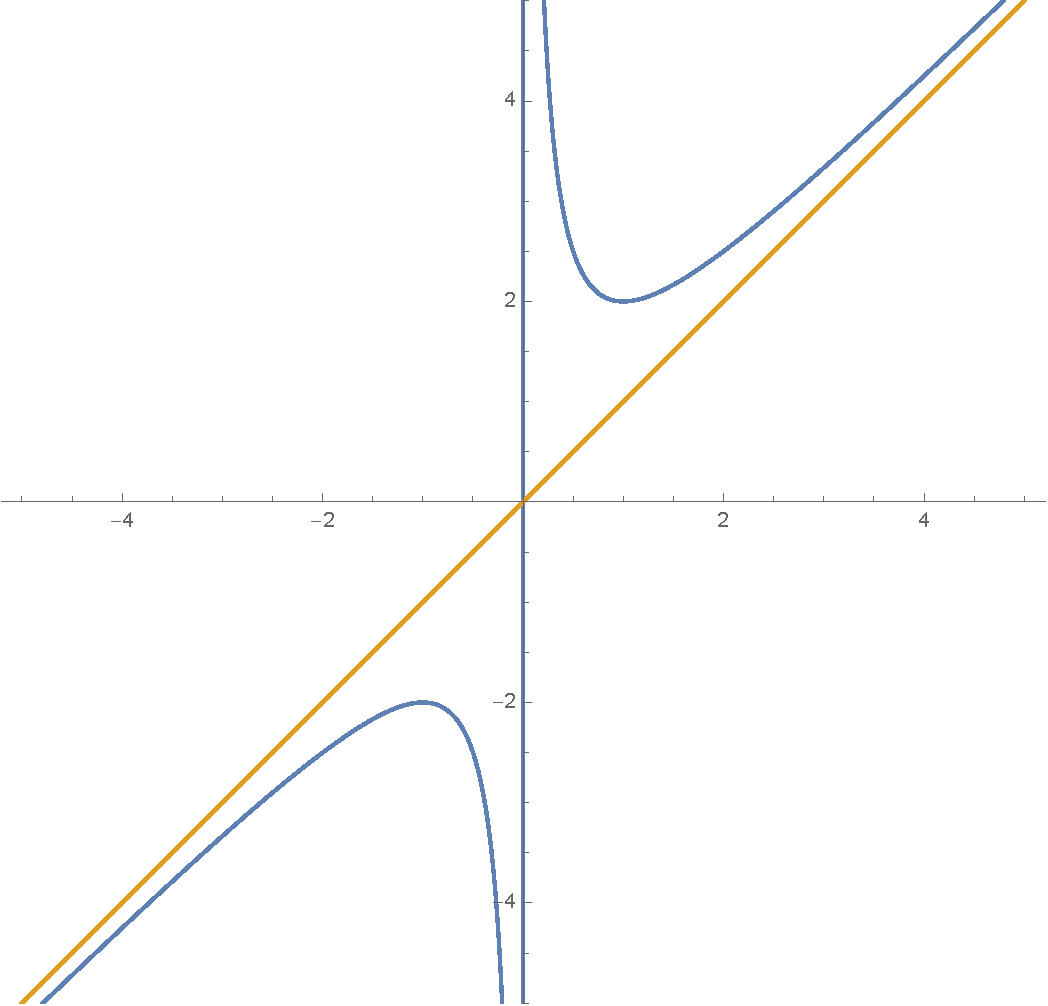
\includegraphics[width=7cm]{./images/ch3/x1x.pdf}
	\end{center}
\end{frame}

\begin{frame}
	\linespread{1.5}
	\ba{1.描绘下列函数的图形:(2)$y=e^{-(x-1)^2}$
	}
	
	\begin{center}
		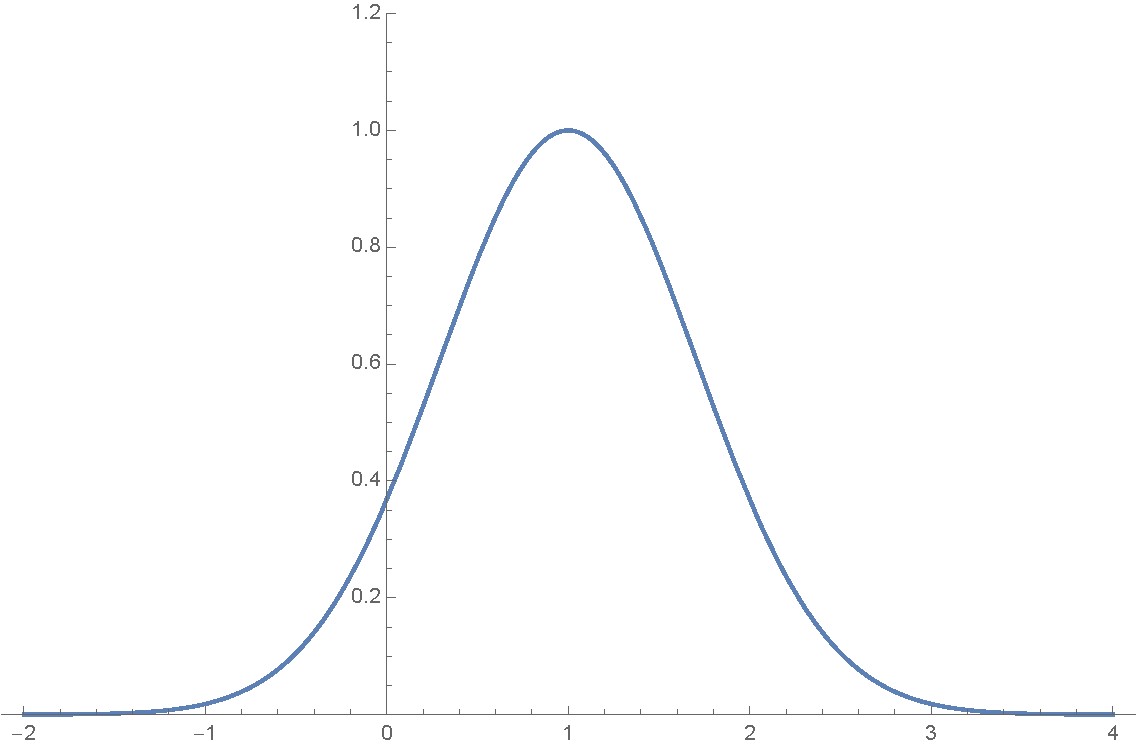
\includegraphics[width=8cm]{./images/ch3/e-2x.pdf}
	\end{center}
\end{frame}